\documentclass{article}
\usepackage[utf8]{inputenc}

\usepackage{graphicx}
\usepackage{color}
\usepackage{float}
\usepackage[pdf]{graphviz}

\usepackage{geometry}
\geometry{hmargin=2.5cm,vmargin=1.5cm}

\begin{document}

\begin{figure}[t]
\centering

\includegraphics[width=5cm]{inp_n7.png}
\end{figure}

\title{\vspace{4cm} \textbf{Chaîne de vérification de modèles de processus}}
\author{El Bouzekraoui Younes | MDAA Saad}
\date{\vspace{7cm} Département Sciences du Numérique - Deuxième année \\
2020-2021 }

\maketitle

\newpage
\tableofcontents

\newpage
%%%%%%%%%%%%%%%%%%%%%%%%%%%%%%%%%%%%%%%%%%%%%%%%%%%%%%%%%%%%%%%%%%
\section{Introduction}
Ce mini-projet consiste à produire une chaîne de vérification de modèles de processus \textbf{SimplePDL} dans le but de vérifier leur cohérence,
en particulier pour savoir si le processus décrit peut se terminer ou non. Pour répondre à cette question, nous utilisons les outils de model-checking
définis sur les réseaux de \textbf{Petri} au travers de la boîte à outils Tina. Il nous faudra donc traduire un modèle de processus en un réseau de Petri.

\section{Le Métamodèle \textbf{SimplePDL}}
\subsection{Modelisation du métamodèle}
On a choisi de définir le Métamodèle SimplePDL comme suit (voir \textbf{SimplePDL.ecore}):
\begin{figure}[H]
    \centering
    
\includegraphics[width = 18cm]{SimplePDL.png}
\end{figure}
Notre Métamodèle SimplePDL est composé de : 

\begin{itemize}
    \item Process : le processus qu'on modélise
    \item ProcessElement : une interface pour faire abstraction sur les éléments d'un processus
    \item Guidance : des notes écrites
    \item Workdefinition : une activité ayant un nom de type EString
    \item WorkSequence : une dépendance entre deux activité
    \item Ressource : une ressource ayant un nom de type EString et une quantité de type EInt
    \item Ressource\_Usage : le lien entre une activité et une ressource
\end{itemize}

Pour prendre en compte l'utilisation des ressources on a ajouté les deux classes : \textbf{Ressource} et \textbf{Ressource\_Usage}
qui héritent de \textbf{ProcessElement}, et on a ajouté un attribut a Workdefinition : \textbf{necessary\_ressources} qui est une liste 
des ressources nécessaires pour une activité. Un objet \textbf{Ressource\_Usage} contient un lien vers une activité et un lien vers 
une ressource et la quantité consommé.

\subsection{Contraintes OCL}
Afin de capturer plus de contraintes On a ajouté les règles ocl suivantes (voir \textbf{SimplePDL.ocl}):
\begin{itemize}
    \item une dépendance ne peut pas être réflexive.
    \item deux sous-activités différentes d’un même processus ne peuvent pas avoir le même nom.
    \item le nom d’une activité doit être composé d’au moins un caractère.
    \item le nom d’une resource doit être composé d’au moins un caractère.
    \item deux ressources ne peuvent pas avoir le même nom.
    \item la quantité d'une ressource doit être $\geq$ 0
    \item la quantité d'une ressource usé doit être $>$ 0
    \item la quantité d'un ressource utilisé par une activité doit être inférieur ou égale à la quantité disponible
\end{itemize}

\section{Le Métamodèle \textbf{PetriNet}}
\subsection{Modelisation du métamodèle}
On a choisi de définir le Métamodèle SimplePDL comme suit (voir \textbf{PetriNet.ecore}):
\begin{figure}[H]
    \centering
    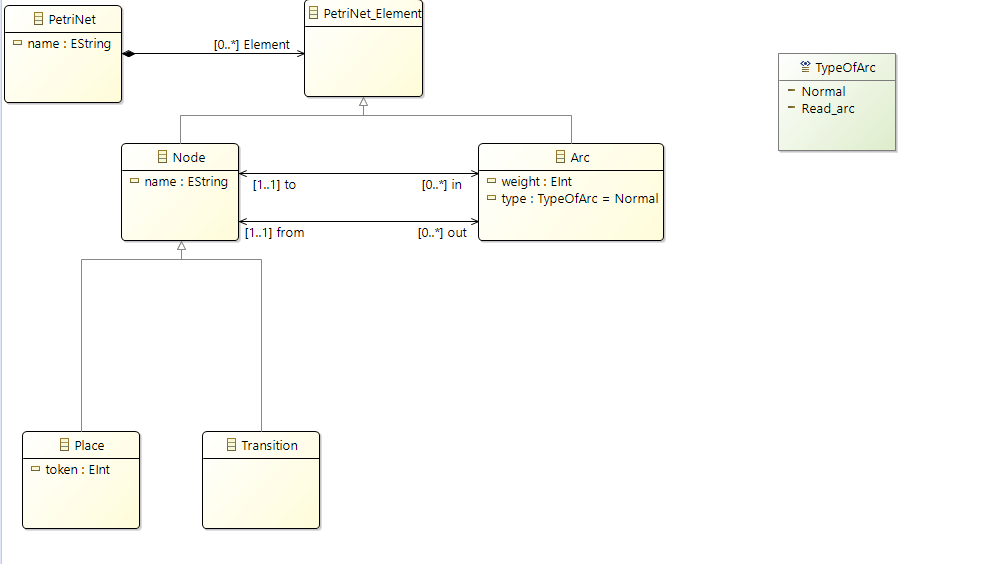
\includegraphics[width = 18cm]{PetriNet.png}
\end{figure}
Notre Métamodèle PetriNet est composé de : 
\begin{itemize}
    \item PetriNet : le réseau petri qu'on modélise
    \item PetriNet\_Element : une interface pour faire abstraction sur les éléments d'un réseau petri
    \item Node : une interface pour faire abstraction sur une place et une transition
    \item Arc : modélise le lien entre une place et une transition de type Normal ou Read\_arc
    \item Place 
    \item Transition 
\end{itemize}

\subsection{Contraintes OCL}
Afin de capturer plus de contraintes On a ajouté les règles ocl suivantes (voir \textbf{PetriNet.ocl}):
\begin{itemize}
    \item un arc doit suivre le modele suivant place arc transition arc place.
    \item le poids d'un arc ne peut pas être nul (sinon l'arc ne sert à rien).
    \item le nombre des jetons dans une place est positive.
    \item le nom d’une node doit être composé d’au moins un caractère.
    \item deux nodes différente peuvent pas avoir le même nom.
    \item le nom d’un réseau Petri doit être composé d’au moins un caractère.
\end{itemize}

\section{Un éditeur graphique SimplePDL}

\section{Syntaxe concrète textuelle de SimplePDL avec Xtext}
Xtext consiste à définir une syntaxe concrète textuelle pour un DSML au travers d’une grammaire, et il permet aussi 
de construire un métamodèle conforme à la syntaxe concrète décrite 
\subsection{Définition de la syntaxe PDL1:}
(voir \textbf{PDL1.xtext}) \\
Un exemple de la syntaxe textuelle généré est donnée dans l'exemple ci-dessous.
\begin{verbatim}
    process dev {
        rs concepteur qt 3
        rs developpeur qt 2
        rs machine qt 4
        rs redacteur qt 2
        rs testeur qt 2
        
        wd Conception needs to get 2 of concepteur get 1 of machine
        wd RedactionDoc needs to get 1 of machine get 1 of redacteur
        wd Programmation needs to get 2 of developpeur get 3 of machine
        wd RedactionTests needs to get 2 of machine get 1 of testeur
        
        ws f2f from Conception to RedactionDoc
        ws s2s from Conception to RedactionDoc
        ws f2f from Conception to Programmation
        ws s2s from Conception to RedactionTests
        ws f2f from Programmation to RedactionTests
    }
\end{verbatim}
Le métamodèle généré à partir de cette syntaxe textuelle est donnée ci-dessous : 
\begin{figure}[H]
    \centering
    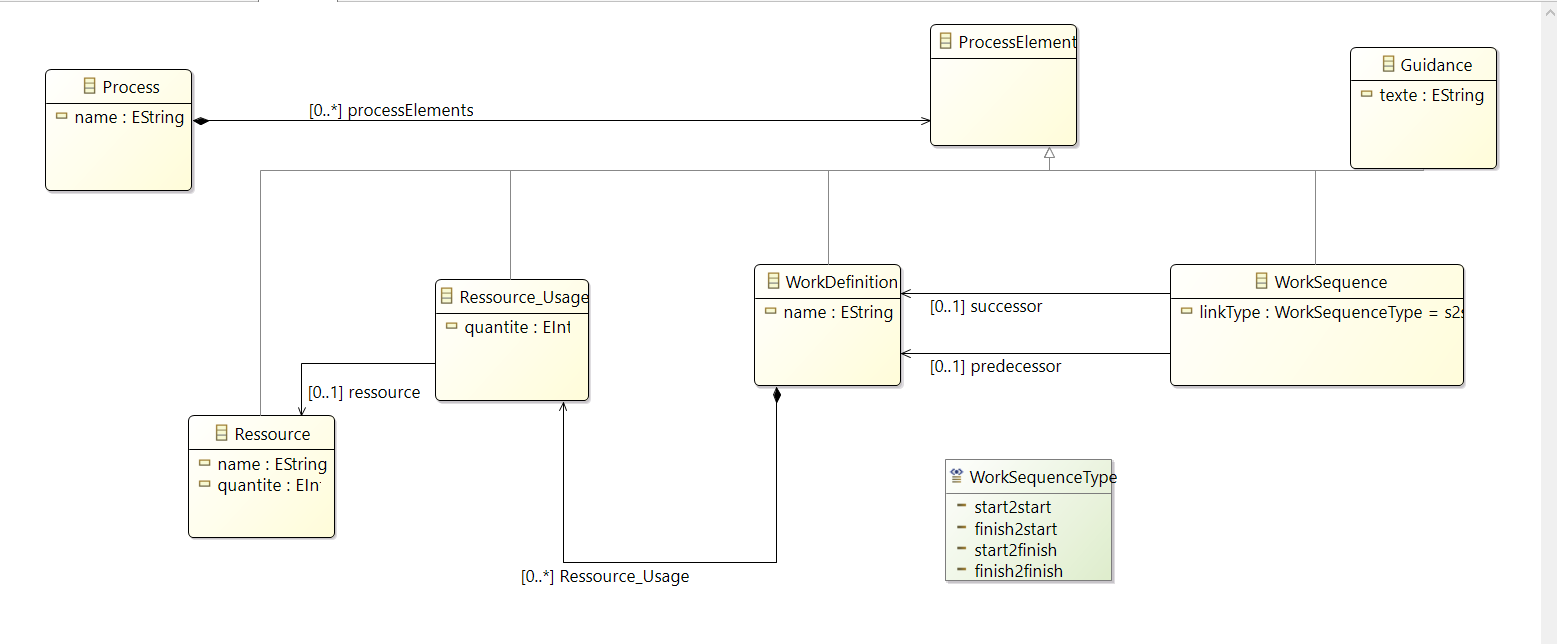
\includegraphics[width = 18cm]{SimplePDLXtext.png}
\end{figure}
Ce métamodèle est différent de celui qu'on definit au début.
\section{Transformation SimplePDL vers PetriNet en utilisant EMF/Java}
EMF nous permet de générer les classes Java a partir des modèles SimplePDL et PetriNet, ce qui nous permet de définir une transformation
de SimplePDL vers PetriNet en utilisant Java (voir \textbf{SimplePDL2PetriNet.java})
\subsection{Principe de la transformation d’un modèle de processus en réseau de Petri}
Le principe de la transformation d’un modèle SimplePDL en Réseau de Pétri est le suivant :
\begin{itemize}
    \item Un élément Process devient un élément PetriNet.
    \item Une WorkDefinition devient 4 places ready, started, running et finished et deux transitions start et finish.
    \item Une WorkSequence devient un read arc entre une place de l’activité précédente (started ou finished) et une transition de l’activité cible (start ou finish).
    \item Une Ressource devient une place, le nombre de jetons indique la quantité
    \item Un Ressource\_Usage devient deux arc , un arc (allocation) dont la multiplicité est la quantité utilisé allant de la place ressource vers la transition start de l'activité . et l'autre arc (déallocation)allant de la transition finish vers la place ressource
\end{itemize}

\section{Transformation SimplePDL vers PetriNet en utilisant ATL}
ATL est un langage et une boîte à outils de transformation de modèles. Dans le domaine de l'ingénierie pilotée par les modèles, 
ATL fournit des moyens de produire un ensemble de modèles cibles à partir d'un ensemble de modèles source.
\subsection{Principe de la transformation d’un modèle de processus en réseau de Petri}
On a suivit les mèmes principes décrit dans la transformation java, on a définit les règles suivantes : (voir \textbf{SimplePDL2PetriNet.atl}). \\
Vue qu'on a pas définit précédemment une référence opposite entre PetriNet et PetriNetElement l'opération suggéré lors du tp: 
\begin{verbatim}
    net <- wd.getProcess())
\end{verbatim}
n'est pas possible, donc on a ajouté les places / transitions / arc crées lors de la règle 
\begin{verbatim}
    Process2PetriNet {..}
\end{verbatim}
en utilisant 
\begin{verbatim}
thisModule.resolveTemp(..)
\end{verbatim}
\section{Tests de la transformation M2M}
\subsection{Modèle simple}
On commence par tester la transformation sur un modèle simple (voir \textbf{pdl-simple.xmi}), il est composé de 2 activités : (cook et eat)
,une dépendance de type finishTostart entre les 2 activités, et une ressource plat utilisé par cook et eat.
\begin{figure}[H]
    \centering
    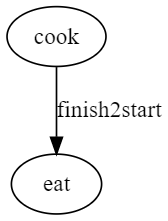
\includegraphics[width = 3cm]{pdl-simple.png}
\end{figure}
la transformation nous donne le modèle Petrinet suivant:
\begin{figure}[H]
    \centering
    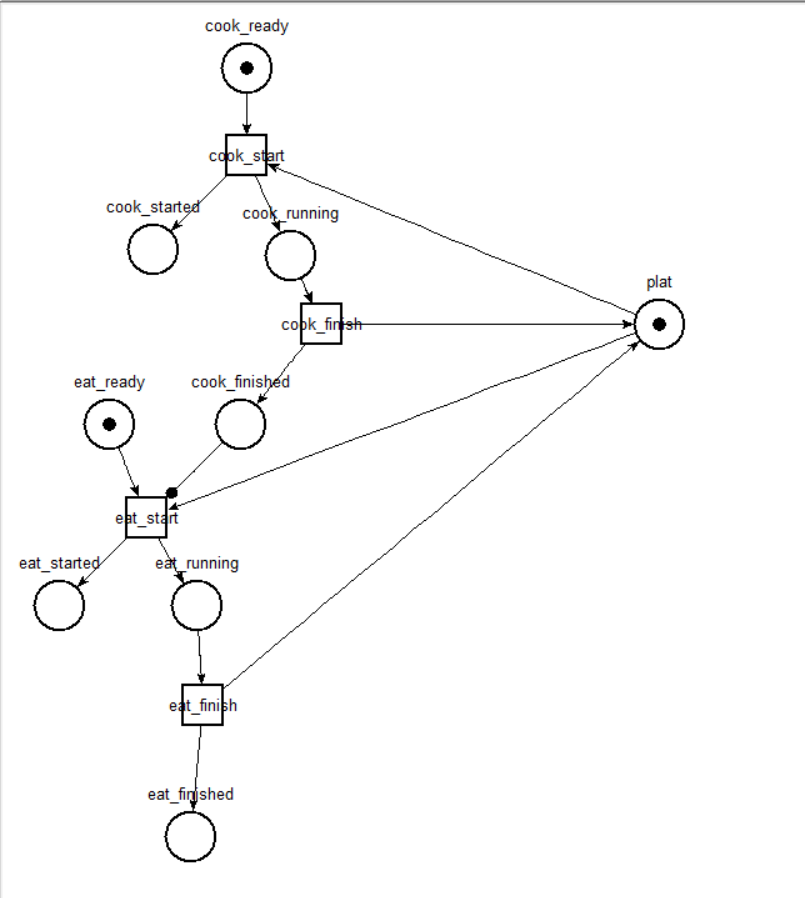
\includegraphics[width = 10cm]{net-simple.png}
\end{figure}
en utilisant le stepper analyser de l'outil netdraw notre modèle Petrinet semble avoir le comportement correcte.
\subsubsection{Validation de la transformation avec l'outil selt}
On génère les propriétés de sûreté du modèle conforme a SimplePDL et on vérifie la terminaision 
du process en utilisant l'outil Acceleo (\textbf{voir toLTL.mtl})
pour vérifier que les invariants sur le modèle de processus sont préservés sur le modèle de réseau de Petri correspondant. \\
fichier simple.ltl généré :
\begin{verbatim}
    op finished = cook_finished /\  eat_finished  ; 
    [] (finished => dead);
    [] <> dead;
    [] (dead => finished);
    - <> finished;
    
    [] (cook_ready + cook_running + cook_finished = 1);
    [] (cook_ready + cook_started = 1);
    [] (eat_ready + eat_running + eat_finished = 1);
    [] (eat_ready + eat_started = 1);
\end{verbatim}
Les 5 premières lignes c'est pour vérifier si toutes les activités se terminent (on attend que propriété sera fausse et le model 
checker exhibera un contre-exemple qui correspond à un scénario qui correspond à la terminaison du processus) \\
Les dernières lignes c'est pour vérifier chaque activité est soit non commencée, soit en cours, soit terminée.
Resultat du verification :
\begin{figure}[H]
    \centering
    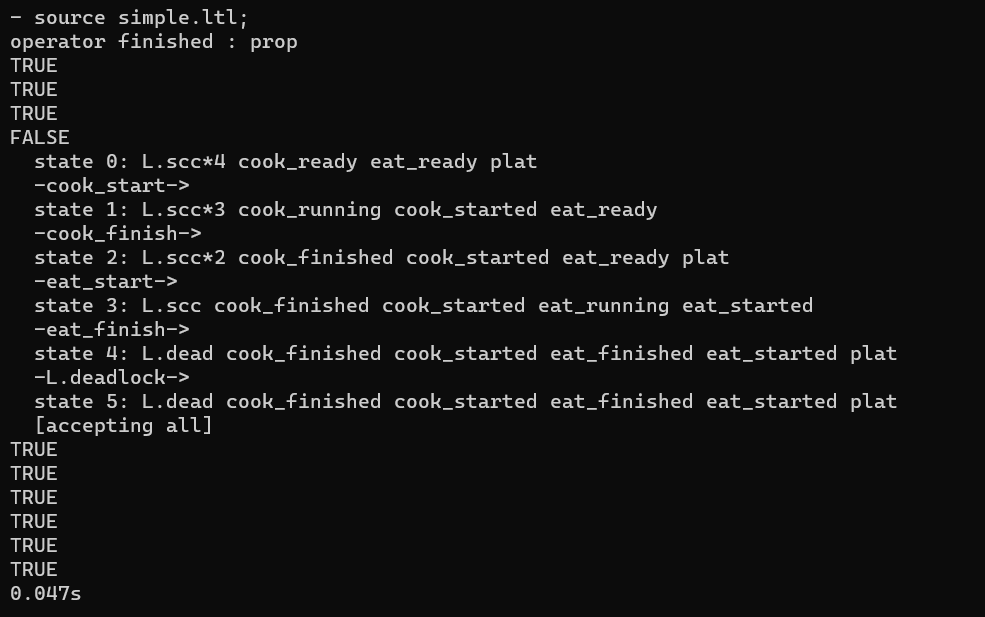
\includegraphics[width = 15cm]{selt-simple.png}
\end{figure}
\subsection{Modèle sujet}
On teste la transformation sur le modèle inspiré de SPEM donnée dans le sujet :
\begin{figure}[H]
    \centering
    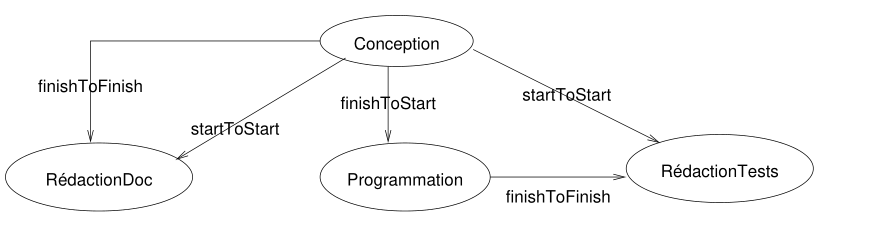
\includegraphics[width = 15cm]{pdl-sujet.png}
\end{figure}
la transformation nous donne le modèle Petrinet suivant:
\begin{figure}[H]
    \centering
    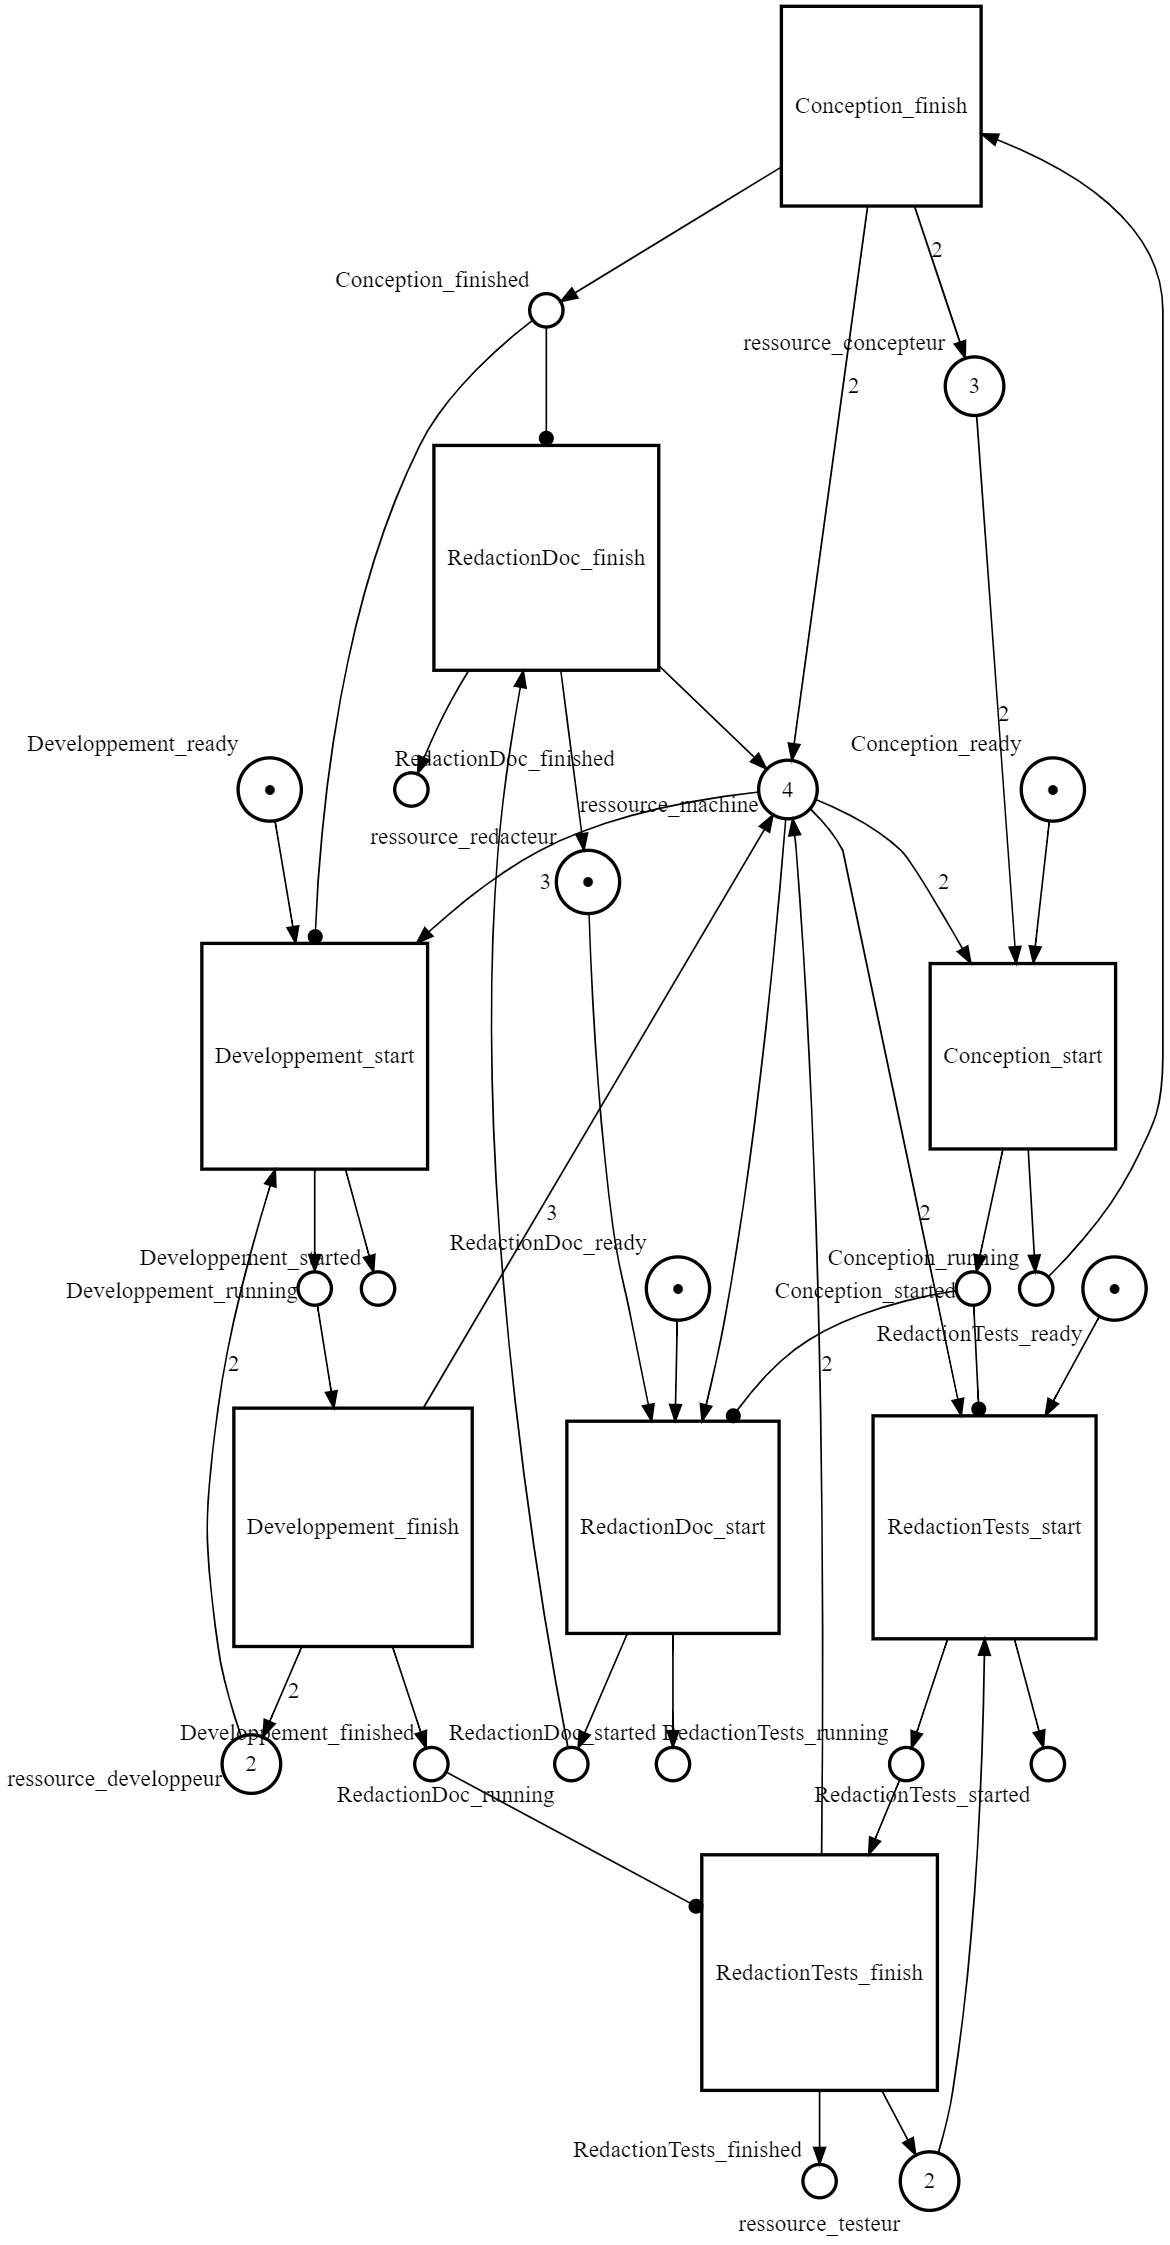
\includegraphics[width = 10cm]{net-sujet.png}
\end{figure}
On remarque que le process simple termine toujours
\subsubsection{Validation de la transformation avec l'outil selt}
fichier simple.ltl généré :
\begin{verbatim}
    op finished = Conception_finished /\  RedactionDoc_finished /\  Developpement_finished /\  RedactionTests_finished  ; 
    [] (finished => dead);
    [] <> dead;
    [] (dead => finished);
    - <> finished;
    
    [] (Conception_ready + Conception_running + Conception_finished = 1);
    [] (Conception_ready + Conception_started = 1);
    [] (RedactionDoc_ready + RedactionDoc_running + RedactionDoc_finished = 1);
    [] (RedactionDoc_ready + RedactionDoc_started = 1);
    [] (Developpement_ready + Developpement_running + Developpement_finished = 1);
    [] (Developpement_ready + Developpement_started = 1);
    [] (RedactionTests_ready + RedactionTests_running + RedactionTests_finished = 1);
    [] (RedactionTests_ready + RedactionTests_started = 1);
\end{verbatim}
Resultat du verification :
\begin{figure}[H]
    \centering
    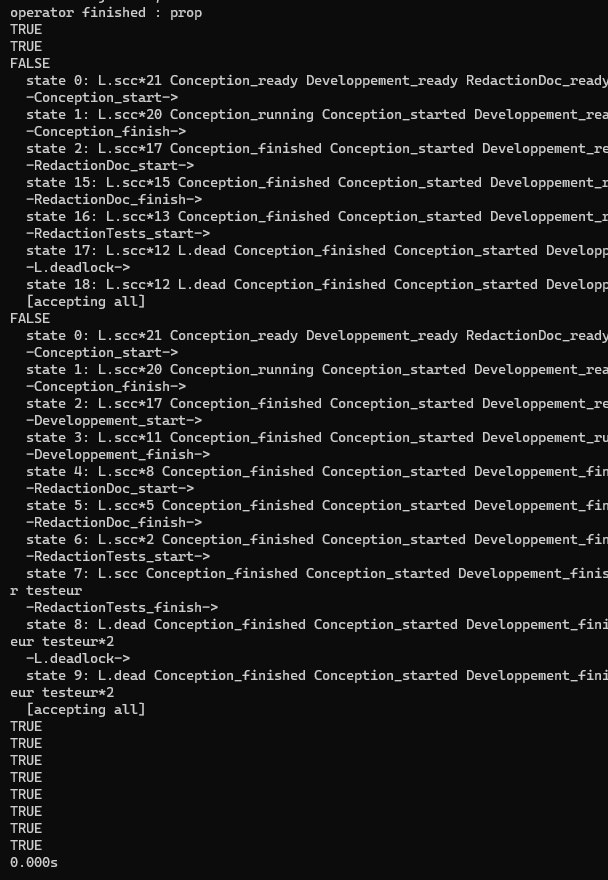
\includegraphics[width = 15cm]{selt-sujet.png}
\end{figure}
On remarque que le process sujet peut terminer


\section{Transformation PetriNet vers Tina/dot en utilisant Acceleo}
Acceleo est un générateur de code source de la fondation Eclipse permettant de mettre en ouvre 
l'approche MDA (Model driven architecture) pour réaliser des applications à partir de modèles basés sur EMF \\
voir \textbf{toTINA.mtl} et voir \textbf{toDOT.mtl}
\subsection{Tests de la transformation M2T}
\subsubsection{Réseau saisons}
\begin{figure}[H]
    \centering
    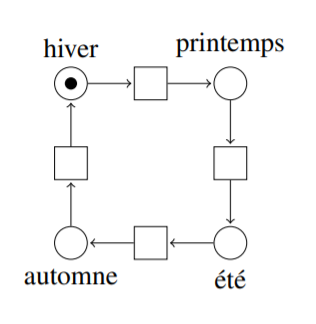
\includegraphics[width = 5cm]{net-saisons.png}
\end{figure}
la transformation nous donne le texte tina suivant :
\begin{verbatim}
    net saisons
    pl Hiver (1)
    pl Printemps (0)
    pl Ete (0)
    pl Automne (0)

    tr h2p  Hiver ->  Printemps
    tr p2e  Printemps ->  Ete
    tr e2a  Ete ->  Automne
    tr a2h  Automne ->  Hiver
\end{verbatim}
la transformation nous donne le diagramme dot suivant :
\begin{figure}[H]
    \centering
    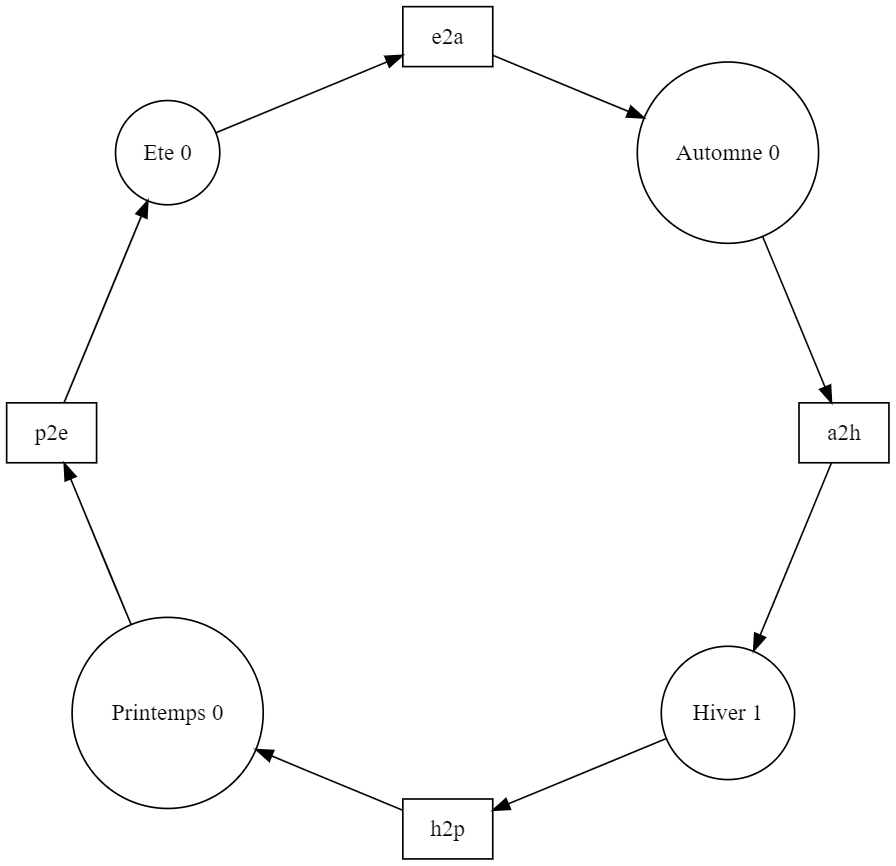
\includegraphics[width = 10cm]{dot-saisons.png}
\end{figure}
\subsubsection{Réseau producteur consomateur}
\begin{figure}[H]
    \centering
    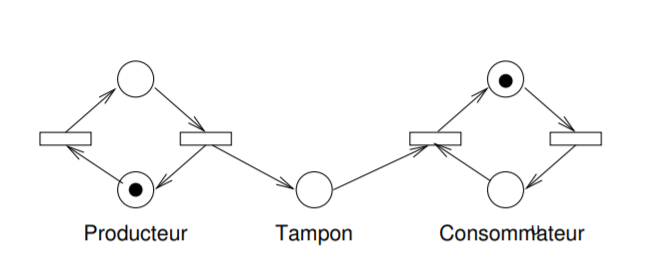
\includegraphics[width = 10cm]{net-prodcons.png}
\end{figure}
la transformation nous donne le texte tina suivant :
\begin{verbatim}
    net prodcons
    pl P1 (1)
    pl P2 (0)
    pl Tampon (0)
    pl C1 (0)
    pl C2 (1)
    
    tr P1P2  P1 ->  P2
    tr P2P1  P2 ->  P1 Tampon
    tr TC2  Tampon C1 ->  C2
    tr C2C1  C2 ->  C1
\end{verbatim}
la transformation nous donne le diagramme dot suivant :
\begin{figure}[H]
    \centering
    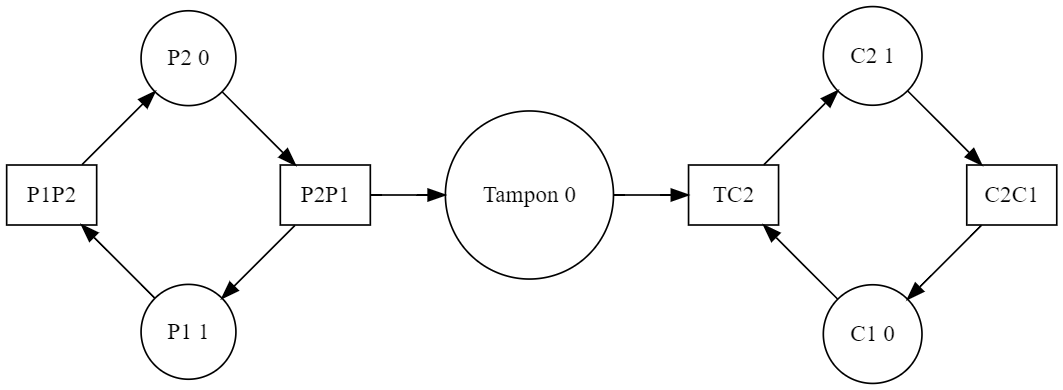
\includegraphics[width = 15cm]{dot-prodcons.png}
\end{figure}
\end{document}